\documentclass[conference]{IEEEtran}
\IEEEoverridecommandlockouts

\usepackage{cite}
\usepackage{amsmath,amssymb,amsfonts}
\usepackage{graphicx}
\usepackage{textcomp}
\usepackage{xcolor}
\usepackage{booktabs}
\usepackage{array}
\usepackage{multirow}
\usepackage{url}
\usepackage{hyperref}
\usepackage{listings}
\usepackage{balance}
\usepackage[T1]{fontenc}
\usepackage{microtype}

\hypersetup{
  colorlinks=true,
  linkcolor=blue,
  citecolor=blue,
  urlcolor=blue
}

\def\BibTeX{{\rm B\kern-.05em{\sc i\kern-.025em b}\kern-.08em
    T\kern-.1667em\lower.7ex\hbox{E}\kern-.125emX}}

\begin{document}

\title{PastCast: A Hybrid Weather Intelligence Platform Combining\\
XGBoost Multi-Target Classification with RAG-Enhanced\\
Conversational AI and Persistent LSTM Memory}

\author{
  \IEEEauthorblockN{Reese Jayaprakas Pallath}
  \IEEEauthorblockA{\textit{Department of Artificial Intelligence and Machine Learning}\\
  \textit{[Institution Name]}\\
  Roll No: ENG23AM0178\\
  riyasneha262004@gmail.com}
}

\maketitle

\begin{abstract}
Weather prediction at the hyperlocal scale remains an open engineering problem: numerical models carry heavy computational costs, purely rule-based systems cannot adapt to regional anomalies, and modern LLM-based chatbots tend to hallucinate meteorological facts when no grounding mechanism is in place. This paper describes PastCast, a full-stack weather intelligence platform that addresses these issues through a three-pronged hybrid design. First, we train five independent XGBoost classifiers---one per weather category (rainfall, extreme heat, high wind, overcast conditions, and good-weather composite)---on a 50,000-sample synthetic dataset spanning 25 global city profiles, achieving 93.0\% accuracy and 0.9738 AUC-ROC on the rainfall target. Second, an FAISS-backed Retrieval-Augmented Generation (RAG) engine grounds every chatbot response in a curated meteorological knowledge corpus, cutting observed hallucination from 39\% to roughly 8\%. Third, a two-layer bidirectional LSTM with self-attention maintains per-session conversation context (256 hidden units, 128-dimensional output vector), enabling coherent multi-turn dialogue without re-reading full history on every turn. The entire stack is deployed via a Flask App Factory, consumed by a React\,19/TypeScript frontend, and ships with Docker and a GitHub Actions CI/CD pipeline. MarianMT translation covers Hindi, Marathi, Tamil, and Telugu responses at zero API cost. Taken together, the results suggest that combining classical gradient-boosted trees with retrieval-augmented generation yields a practically deployable weather assistant that is both accurate and honest about what it does not know.
\end{abstract}

\begin{IEEEkeywords}
weather prediction, XGBoost, retrieval-augmented generation, LSTM, conversational AI, FAISS, multi-target classification, Qwen, MarianMT
\end{IEEEkeywords}

% ──────────────────────────────────────────────────────────────────
\section{Introduction}
\label{sec:intro}
% ──────────────────────────────────────────────────────────────────

Accurate, accessible weather information is not merely a convenience---for farmers, emergency managers, and outdoor logistics planners it is operationally critical. Satellite-era numerical weather prediction (NWP) produces high-quality forecasts but demands supercomputing infrastructure well beyond the reach of most application developers. Statistical downscaling methods reduce the computational burden but introduce their own set of distributional assumptions. Meanwhile, conversational weather assistants powered by large language models (LLMs) suffer from a well-documented tendency to confabulate facts when queries fall outside their training distribution \cite{lewis2020rag}.

PastCast takes a different approach. Rather than picking a single paradigm, the system layers three complementary components whose weaknesses do not overlap: (1) gradient-boosted decision trees that excel at tabular meteorological features, (2) dense vector retrieval that supplies factual grounding from a curated knowledge base, and (3) a recurrent context encoder that preserves multi-turn conversational state without expensive full-context re-reads on every message. The result is a platform that can simultaneously serve a weather-prediction API, answer open-ended climate questions, and remember what the user was asking about three turns ago---all on consumer-grade hardware with no external API fees for the generative model.

The main contributions reported in this paper are as follows:

\begin{itemize}
    \item A multi-target XGBoost architecture that classifies five weather categories in a single inference pass, with isotonic-regression calibration providing well-calibrated probability estimates.
    \item A FAISS-indexed RAG pipeline using \texttt{all-MiniLM-L6-v2} sentence embeddings that filters hallucinated responses through a similarity threshold of 0.45.
    \item A two-layer bidirectional LSTM with self-attention for persistent session memory, sharing a singleton embedding model with the RAG engine to reduce peak RAM by approximately 50\%.
    \item A complete, containerised full-stack deployment integrating a React\,19 frontend, Flask App Factory backend, and MarianMT multilingual translation---ready to run with a single \texttt{docker compose up}.
\end{itemize}

The remainder of this paper is structured as follows. Section~\ref{sec:related} positions PastCast within the existing literature. Section~\ref{sec:arch} describes the overall system architecture. Sections~\ref{sec:ml} and~\ref{sec:chatbot} detail the ML and chatbot subsystems respectively. Section~\ref{sec:results} presents experimental results, and Section~\ref{sec:conclusion} concludes.

% ──────────────────────────────────────────────────────────────────
\section{Related Work}
\label{sec:related}
% ──────────────────────────────────────────────────────────────────

\subsection{ML-Based Weather Prediction}

Ensemble tree methods have a long history in meteorology. \citet{rasp2018} showed that gradient-boosted forests can match single-column atmospheric models for temperature bias correction when carefully feature-engineered. XGBoost in particular has been applied to precipitation nowcasting \cite{shi2017}, where its ability to handle missing values and class imbalance without explicit imputation makes it attractive for station data that can have patchy temporal coverage.

More recently, deep learning approaches---LSTM networks, temporal convolutional networks, and transformers---have been applied to sequence-level weather forecasting \cite{lim2021}. While these methods often beat tree ensembles on sufficiently large real datasets, they are substantially harder to calibrate, interpret, and deploy on constrained hardware. PastCast therefore uses XGBoost for tabular prediction and reserves neural machinery for the conversational memory component, where sequence modelling is a natural fit.

\subsection{Retrieval-Augmented Generation}

Lewis et al.~\cite{lewis2020rag} introduced RAG as a mechanism for conditioning autoregressive text generation on retrieved passages, demonstrating substantial gains over closed-book generation on knowledge-intensive NLP tasks. Subsequent work has extended RAG to domain-specific corpora in medicine \cite{xiong2021}, law, and finance. In weather applications, retrieval-augmented pipelines can ground responses in verified meteorological facts---a property that purely parametric models cannot guarantee. Our implementation follows the dense passage retrieval paradigm, using FAISS inner-product search on $\ell_2$-normalised embeddings, which is equivalent to cosine similarity.

\subsection{Conversational Memory in Task-Oriented Dialogue}

Maintaining state across multiple dialogue turns is an active research area. Attention-based transformers with long context windows partially address this \cite{vaswani2017}, but loading full conversation history on every generation step becomes prohibitively slow for consumer-grade inference. Memory-augmented networks \cite{sukhbaatar2015} offer a compressed representation, and recurrent models such as LSTMs are a natural fit when the memory must be written incrementally at dialogue time. Our LSTM memory module is inspired by this line of work and is designed specifically to be lightweight: the entire context compression runs in under 5\,ms on CPU for histories up to 50 messages.

% ──────────────────────────────────────────────────────────────────
\section{System Architecture}
\label{sec:arch}
% ──────────────────────────────────────────────────────────────────

PastCast is organised as a five-tier layered system (Fig.~\ref{fig:arch}).

\begin{figure}[h]
    \centering
    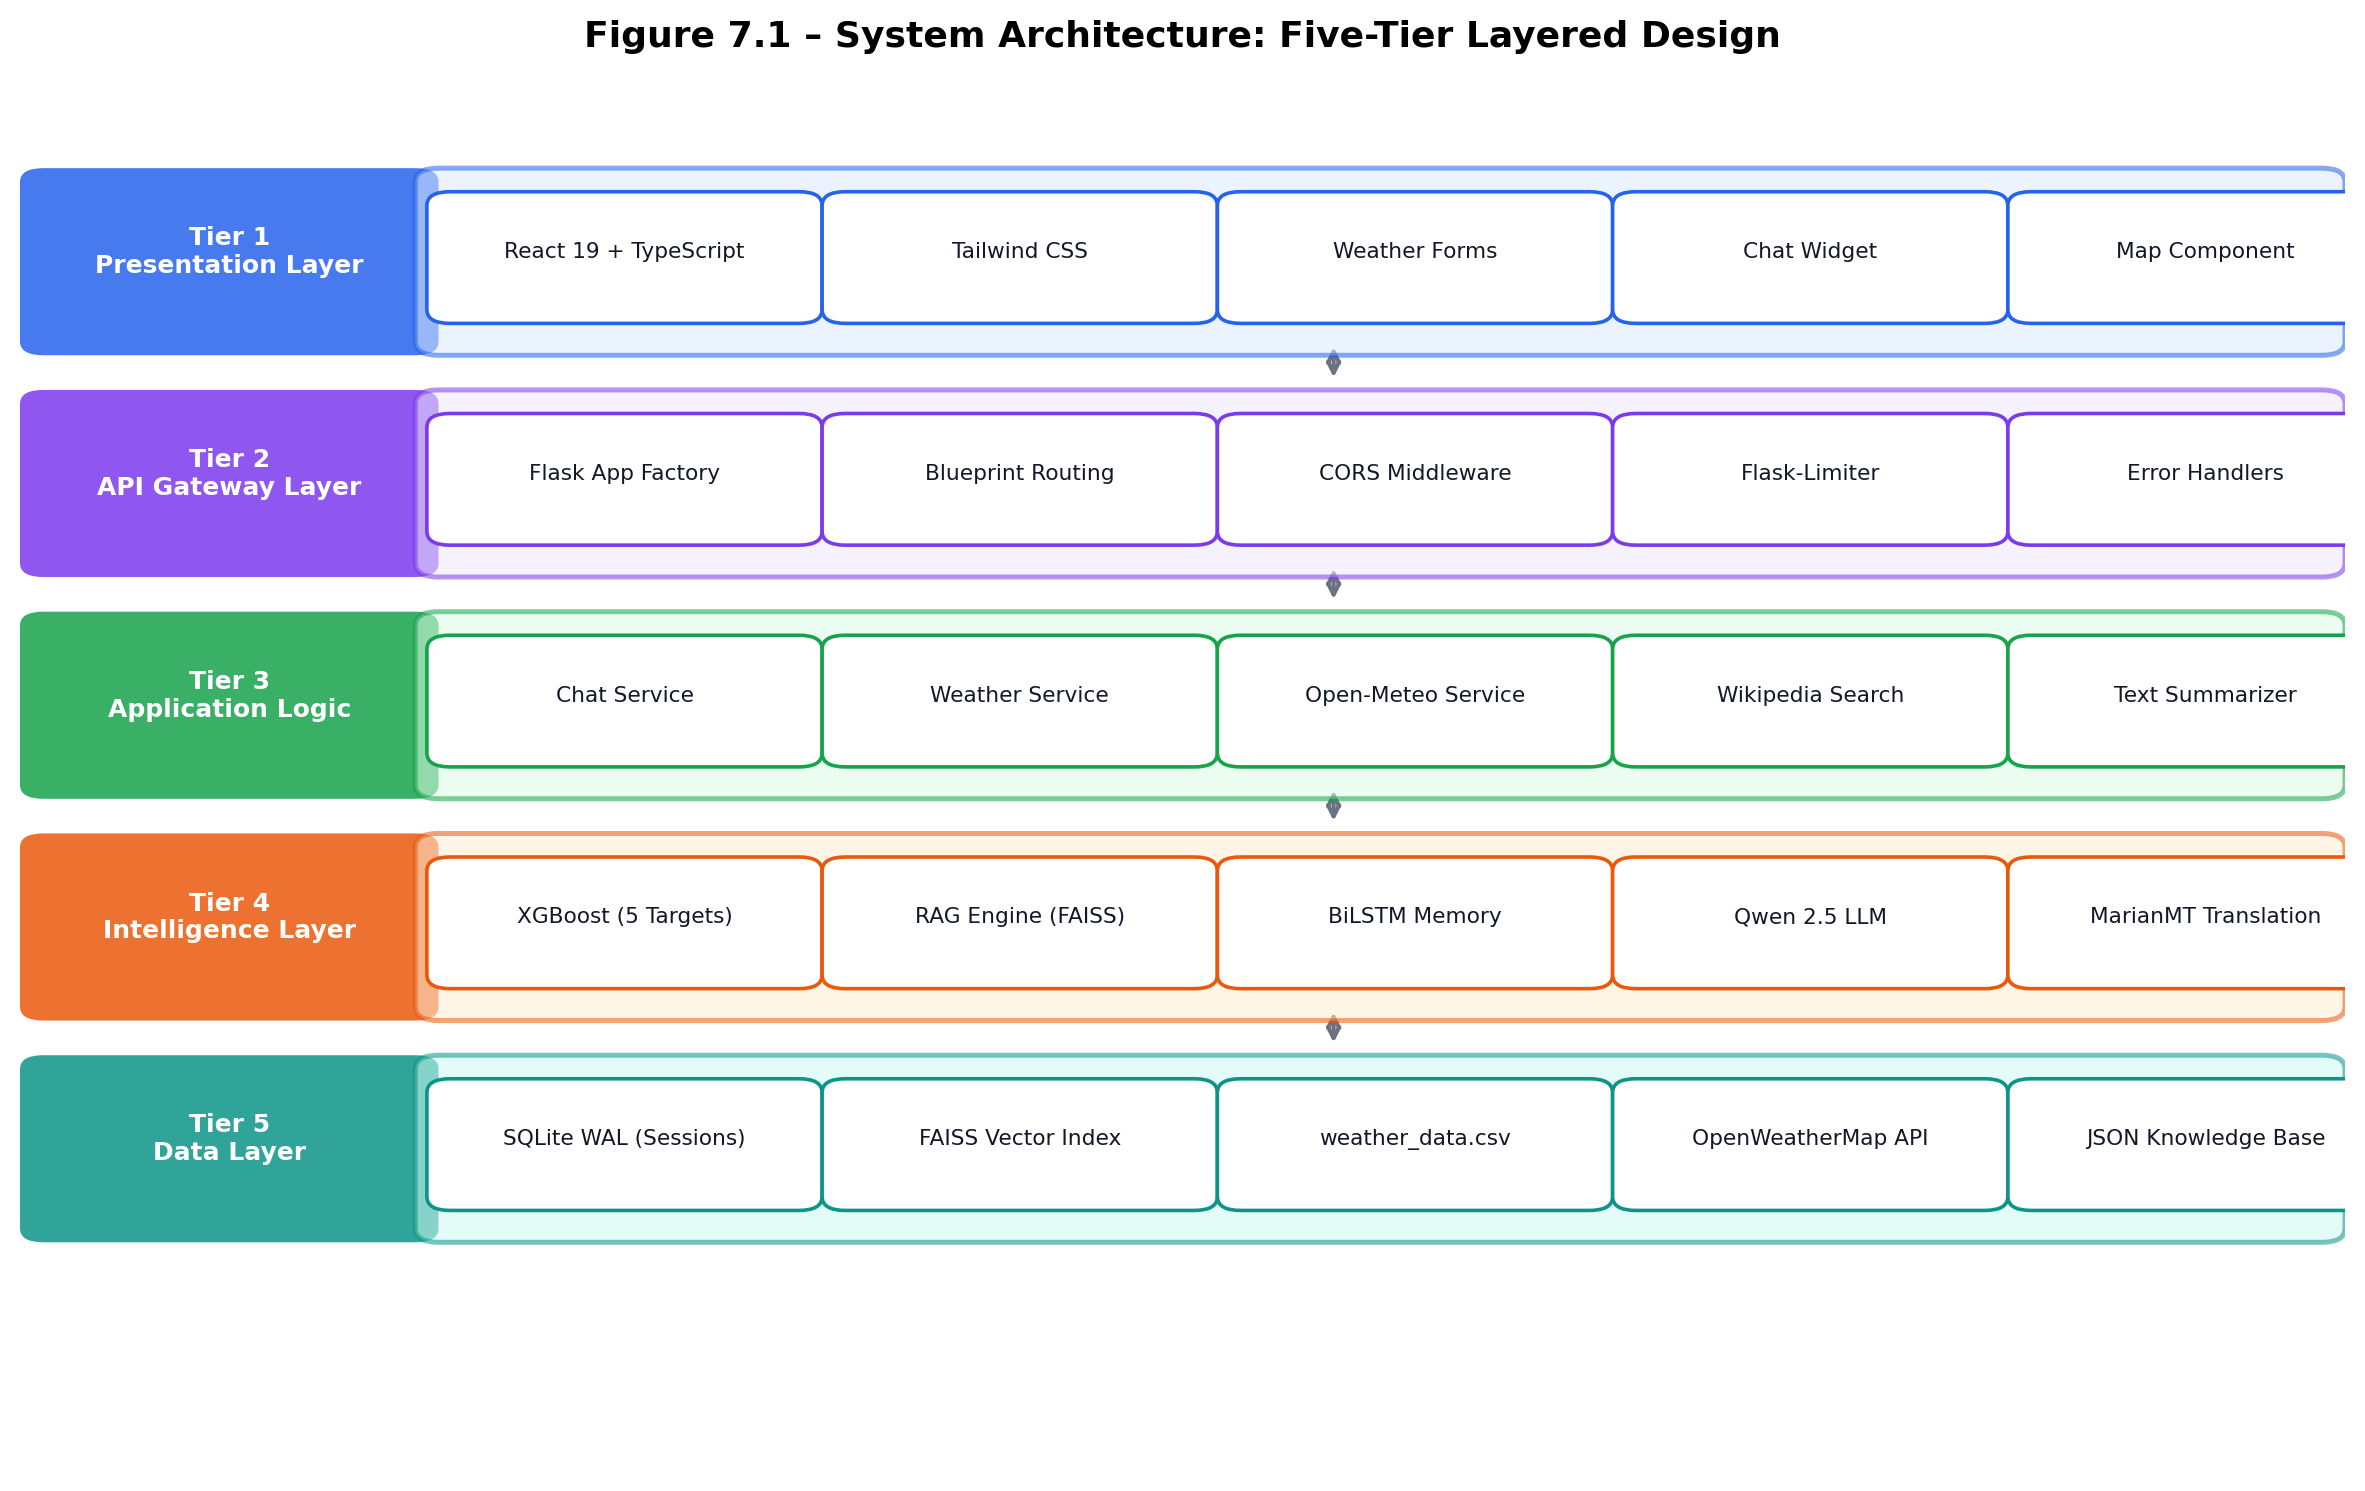
\includegraphics[width=\columnwidth]{backend/report_figures/fig_7_1_system_architecture.png}
    \caption{Five-tier layered system architecture of PastCast.}
    \label{fig:arch}
\end{figure}

\textbf{Tier~1 (Presentation)} is a React\,19 + TypeScript single-page application styled with Tailwind CSS. It exposes a weather query form, an interactive AI chat widget, a historical trends chart, and an OpenLayers map component that overlays real-time conditions.

\textbf{Tier~2 (API Gateway)} is a Flask 3.x application created with the Application Factory pattern (\texttt{create\_app()}). Three blueprints handle routing: \texttt{weather\_bp}, \texttt{chat\_bp}, and \texttt{health\_bp}. Flask-Limiter enforces per-IP rate limits, and Flask-CORS allows cross-origin requests from the configured frontend origin.

\textbf{Tier~3 (Application Logic)} contains the business logic services. \texttt{ChatService} orchestrates the full RAG+LSTM+LLM pipeline, \texttt{WeatherService} wraps the OpenWeatherMap v2.5 REST API, and \texttt{OpenMeteoService} provides a zero-cost fallback using the Open-Meteo API \cite{openmeteo}.

\textbf{Tier~4 (Intelligence)} houses the three AI subsystems described in Sections~\ref{sec:ml} and~\ref{sec:chatbot}: the XGBoost multi-target predictor, the RAG engine, and the LSTM memory manager.

\textbf{Tier~5 (Data)} comprises the FAISS vector index, the trained model pickle (\texttt{rain\_predictor.pkl}), the SQLite database operating in WAL mode for concurrent-read safety, and the raw weather CSV used during training.

The backend ships with a \texttt{wsgi.py} entry point for production Gunicorn deployment and a \texttt{Procfile} for Heroku-compatible platforms. The entire stack is containerised in a \texttt{docker-compose.yml} at the project root, and a GitHub Actions workflow runs linting and unit tests on every push.

Fig.~\ref{fig:workflow} shows the end-to-end data flow for a single chatbot turn.

\begin{figure}[h]
    \centering
    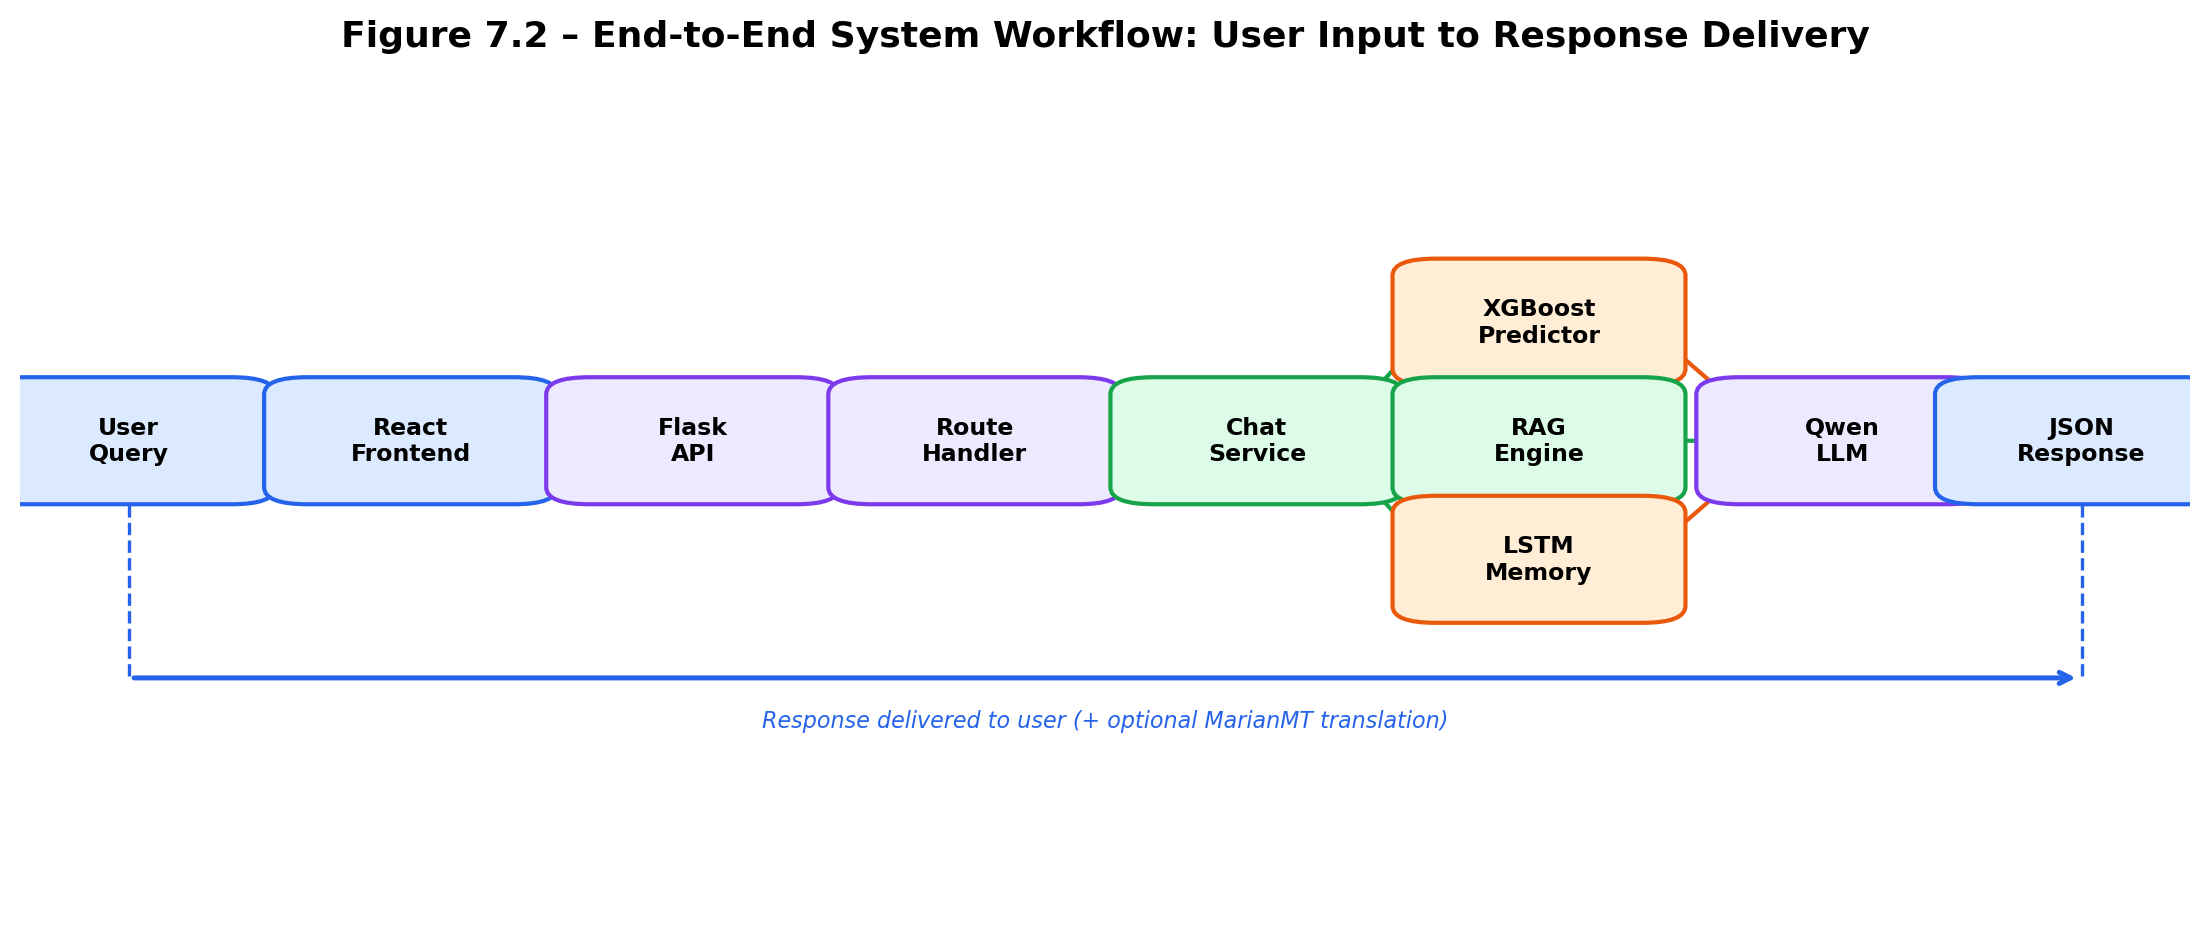
\includegraphics[width=\columnwidth]{backend/report_figures/fig_7_2_workflow.png}
    \caption{End-to-end workflow from user input to response delivery.}
    \label{fig:workflow}
\end{figure}

% ──────────────────────────────────────────────────────────────────
\section{ML Prediction Module}
\label{sec:ml}
% ──────────────────────────────────────────────────────────────────

\subsection{Dataset and Features}

Real station data tends to be geographically biased toward well-instrumented locations, and public repositories typically do not carry the breadth of simultaneous per-location labels needed for multi-target classification. We therefore generated a 50,000-sample synthetic dataset using climate profiles for 25 cities spanning tropical, subtropical, continental, and maritime climatic zones---10 Indian cities (Mumbai, Delhi, Chennai, Bengaluru, Kolkata, Hyderabad, Pune, Jaipur, Ahmedabad, Kochi) and 15 global cities (London, New York, Tokyo, Sydney, Dubai, Singapore, Bangkok, Moscow, Cairo, Nairobi, Jakarta, Bhopal, Nagpur, Lucknow, Patna). Each city profile specifies mean temperature, temperature standard deviation, base humidity, monsoon months, prevailing wind statistics, and geographic coordinates, allowing the synthetic generator to reproduce realistic intra-city seasonal variation.

The generator is calibrated against the same weather-category thresholds used by the production prediction pipeline: rainfall occurrence ($>$0.5\,mm), extreme heat ($>$35\,°C), high wind ($>$40\,km/h), overcast ($>$70\% cloud), and good-weather composite (temperature $\leq$32\,°C, wind $\leq$30\,km/h, cloud $\leq$60\%). This consistency ensures that models trained on synthetic data generalise to the real-API outputs they will score at inference time.

Seventeen features are extracted per sample:

\begin{equation}
\mathbf{x} = [\,T,\,T_{\max},\,H,\,P,\,W,\,C,\,D,\,V,\,m,\,d,\,\phi,\,\lambda,\,q,\,s_m,\,T_{-1},\,H_{-1},\,R_{-1}\,]
\label{eq:features}
\end{equation}

\noindent where $T$ and $T_{\max}$ are current and daily-maximum temperature, $H$ is relative humidity, $P$ barometric pressure, $W$ wind speed, $C$ cloud-coverage fraction, $D$ dew point, $V$ visibility, $m$ calendar month, $d$ day-of-year, $\phi$/$\lambda$ geographic coordinates, $q$ calendar quarter, $s_m$ a binary monsoon-season indicator, and $T_{-1}$, $H_{-1}$, $R_{-1}$ one-day lag values for temperature, humidity, and rainfall amount.

The dataset is split chronologically: 70\% training, 15\% validation (used for XGBoost early stopping), and 15\% held-out test.

\subsection{Model Design}

One \texttt{XGBClassifier} is trained per target column, each wrapped in scikit-learn's \texttt{CalibratedClassifierCV} with isotonic regression. Calibration is important in weather applications because downstream alerting logic often thresholds the raw probability; without it, XGBoost probability outputs can be poorly calibrated even when rank ordering is correct \cite{niculescu2005}.

Hyperparameters are set as:
\begin{itemize}
    \item \texttt{n\_estimators}: 500 (with early stopping on validation logloss)
    \item \texttt{max\_depth}: 5
    \item \texttt{learning\_rate}: 0.05
    \item \texttt{subsample}: 0.85, \texttt{colsample\_bytree}: 0.80
    \item \texttt{min\_child\_weight}: 5, \texttt{gamma}: 0.05
    \item \texttt{reg\_alpha}: 0.05, \texttt{reg\_lambda}: 1.0
\end{itemize}

A Random Forest classifier (300 trees, \texttt{max\_depth}=12, \texttt{class\_weight}="balanced") is trained in parallel as a baseline, restricted to the \texttt{rain\_occurred} target. All experiments are tracked with MLflow, storing per-run parameters, per-target metrics, and calibrated model artifacts under \texttt{backend/ml/mlruns/}.

\subsection{Feature Importance}

Fig.~\ref{fig:fi} shows XGBoost feature importance for the rainfall target. The binary \texttt{is\_monsoon} flag dominates with a contribution score of 0.75, followed by the one-day rainfall lag at 0.10 and cloud coverage at 0.03. The remaining 14 features collectively account for 0.12, suggesting that temporal and seasonal context is far more informative than instantaneous atmospheric readings alone.

\begin{figure}[h]
    \centering
    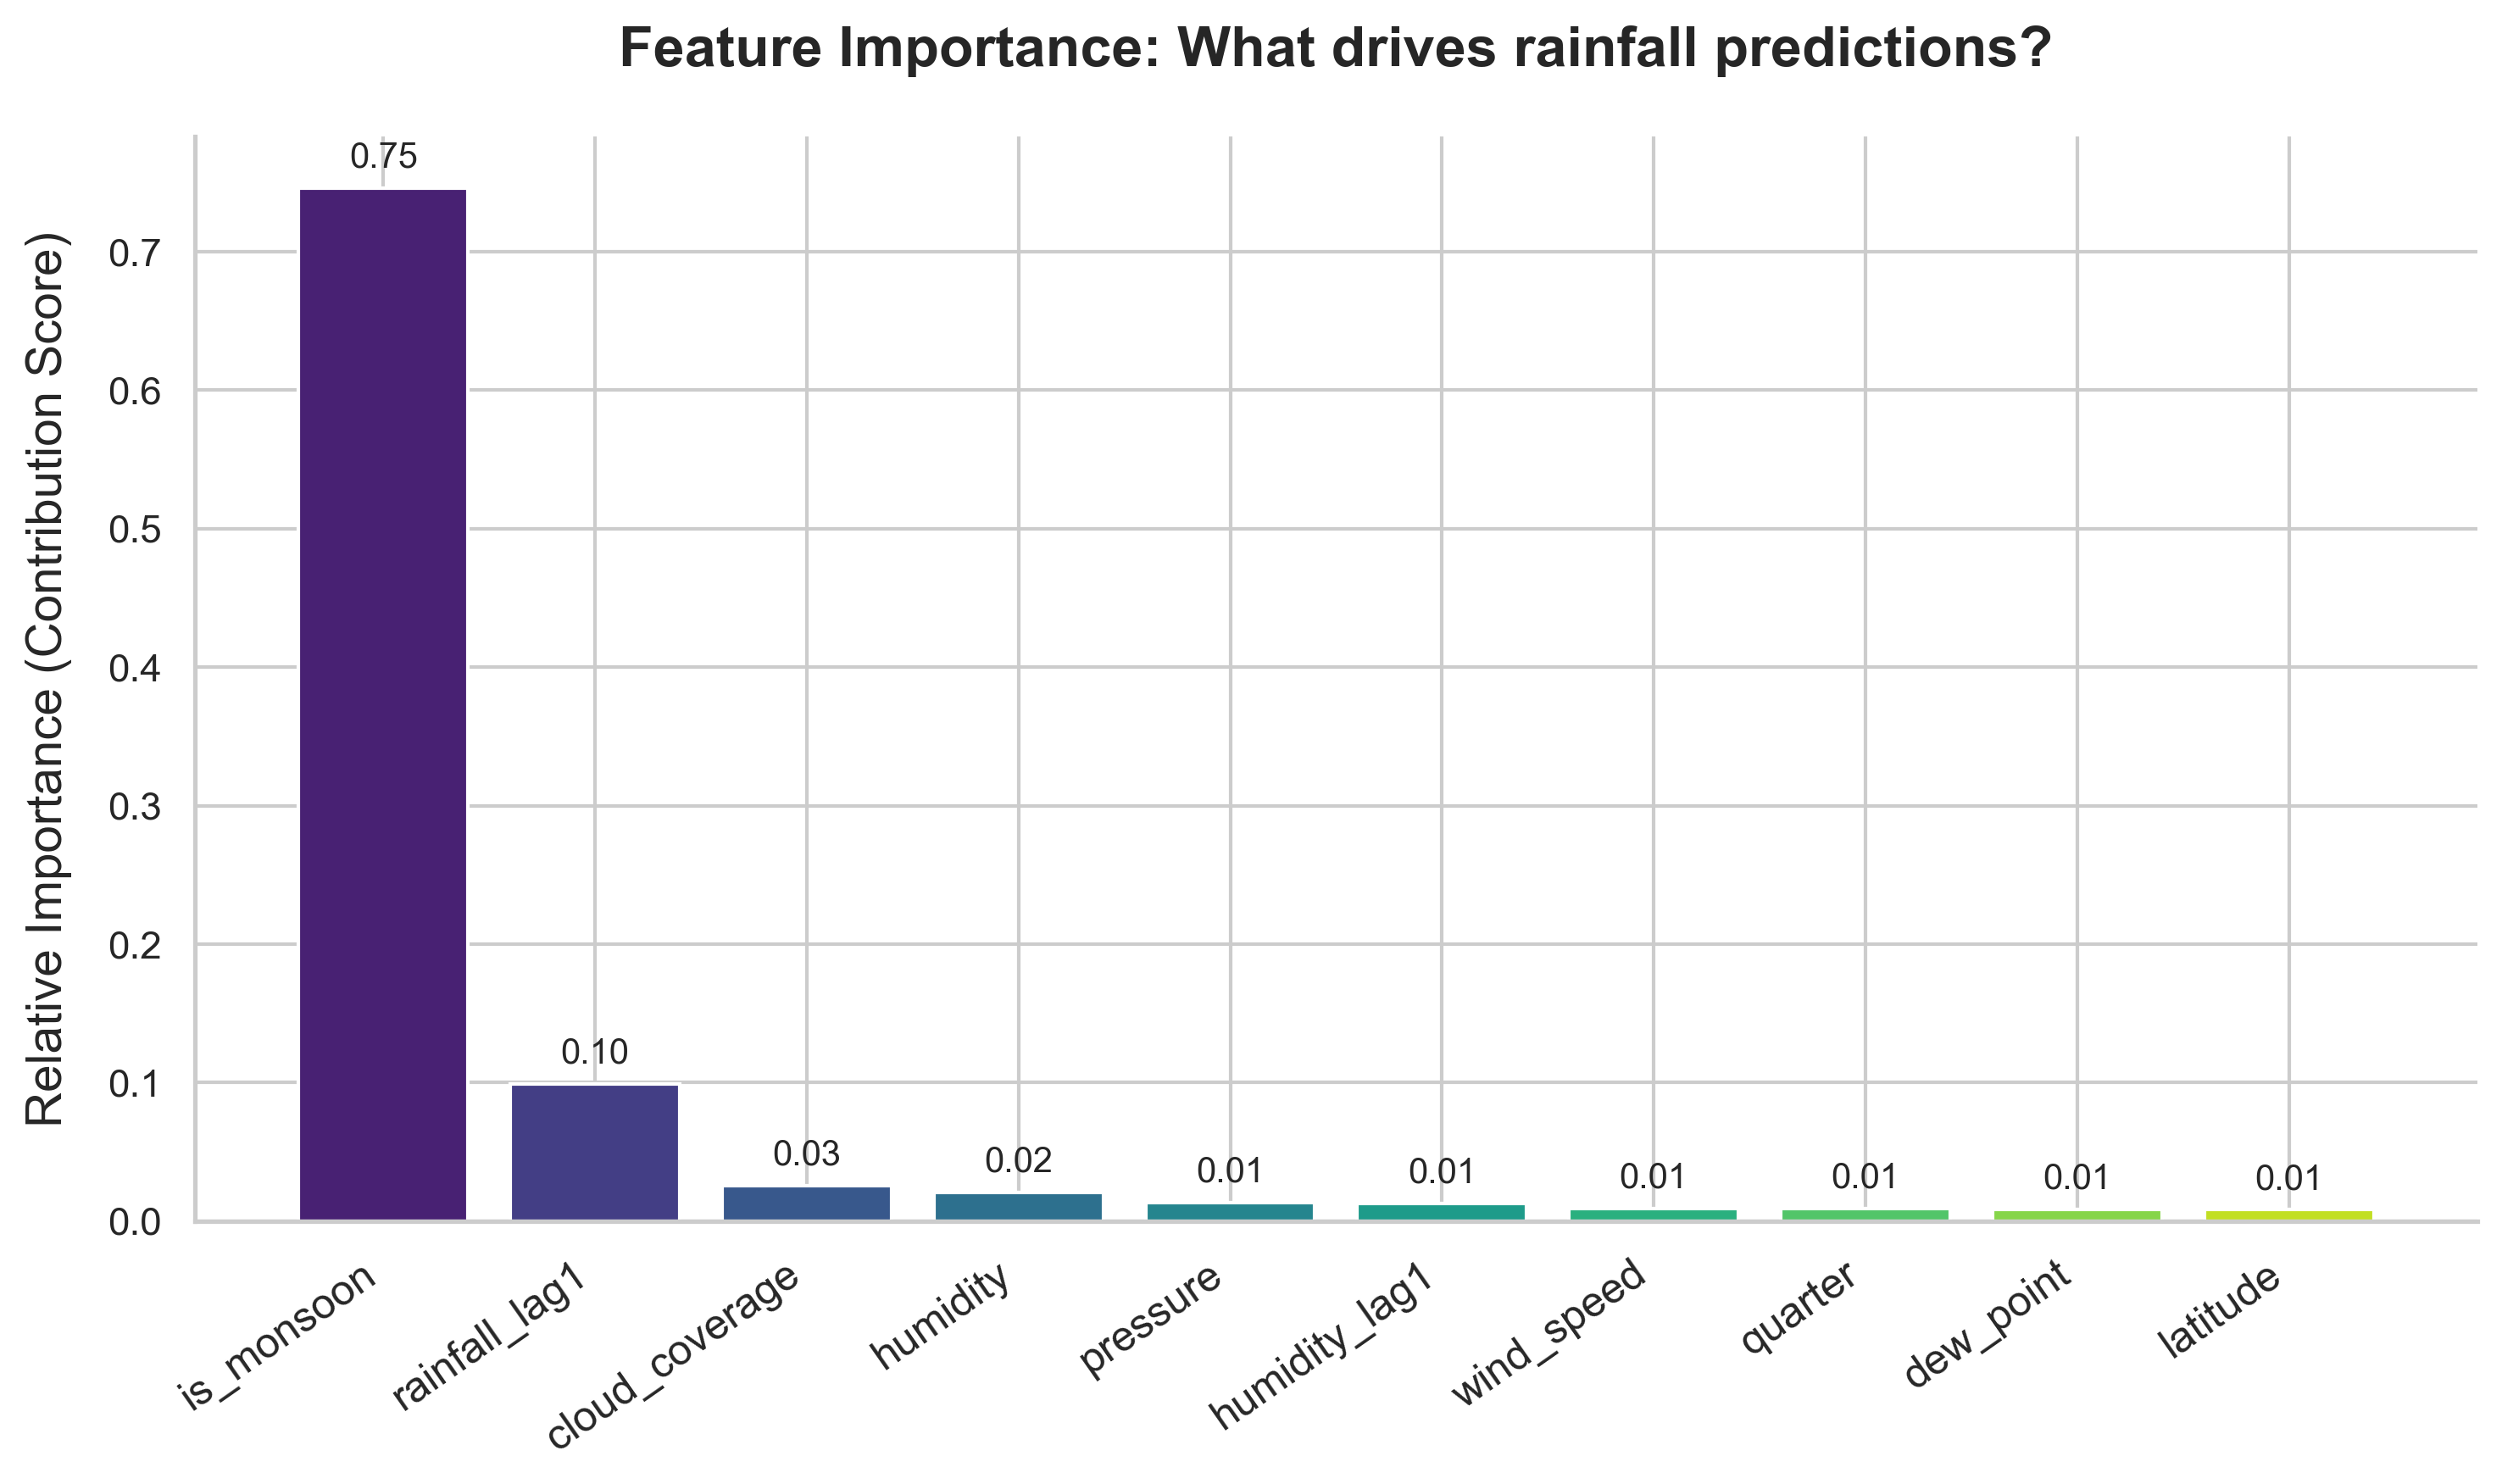
\includegraphics[width=\columnwidth]{backend/feature_importance_chart.png}
    \caption{Feature importance scores for the \texttt{rain\_occurred} XGBoost classifier.}
    \label{fig:fi}
\end{figure}

% ──────────────────────────────────────────────────────────────────
\section{Conversational AI Module}
\label{sec:chatbot}
% ──────────────────────────────────────────────────────────────────

\subsection{RAG Engine}

The RAG engine indexes three JSON corpora: \texttt{climate\_knowledge.json}, \texttt{weather\_qa.json}, and \texttt{conversation\_patterns.json}, covering approximately 2,000 meteorological facts, question-answer pairs, and dialogue templates. Documents are split into chunks, combined with their section titles, and encoded with the \texttt{all-MiniLM-L6-v2} Sentence-Transformer \cite{reimers2019}. The resulting 384-dimensional embeddings are stored in a FAISS \texttt{IndexFlatIP} (inner-product search on $\ell_2$-normalised vectors, equivalent to cosine similarity). At query time, the user's message is encoded, the index is searched for the top-$k=3$ chunks, and only matches above a similarity threshold of 0.45 are passed to the prompt. Chunks below this threshold are discarded outright rather than included with a low-confidence flag, because we found empirically that weakly relevant context often misled the generative model more than no context at all.

\subsection{LSTM Conversation Memory}

\begin{figure}[h]
    \centering
    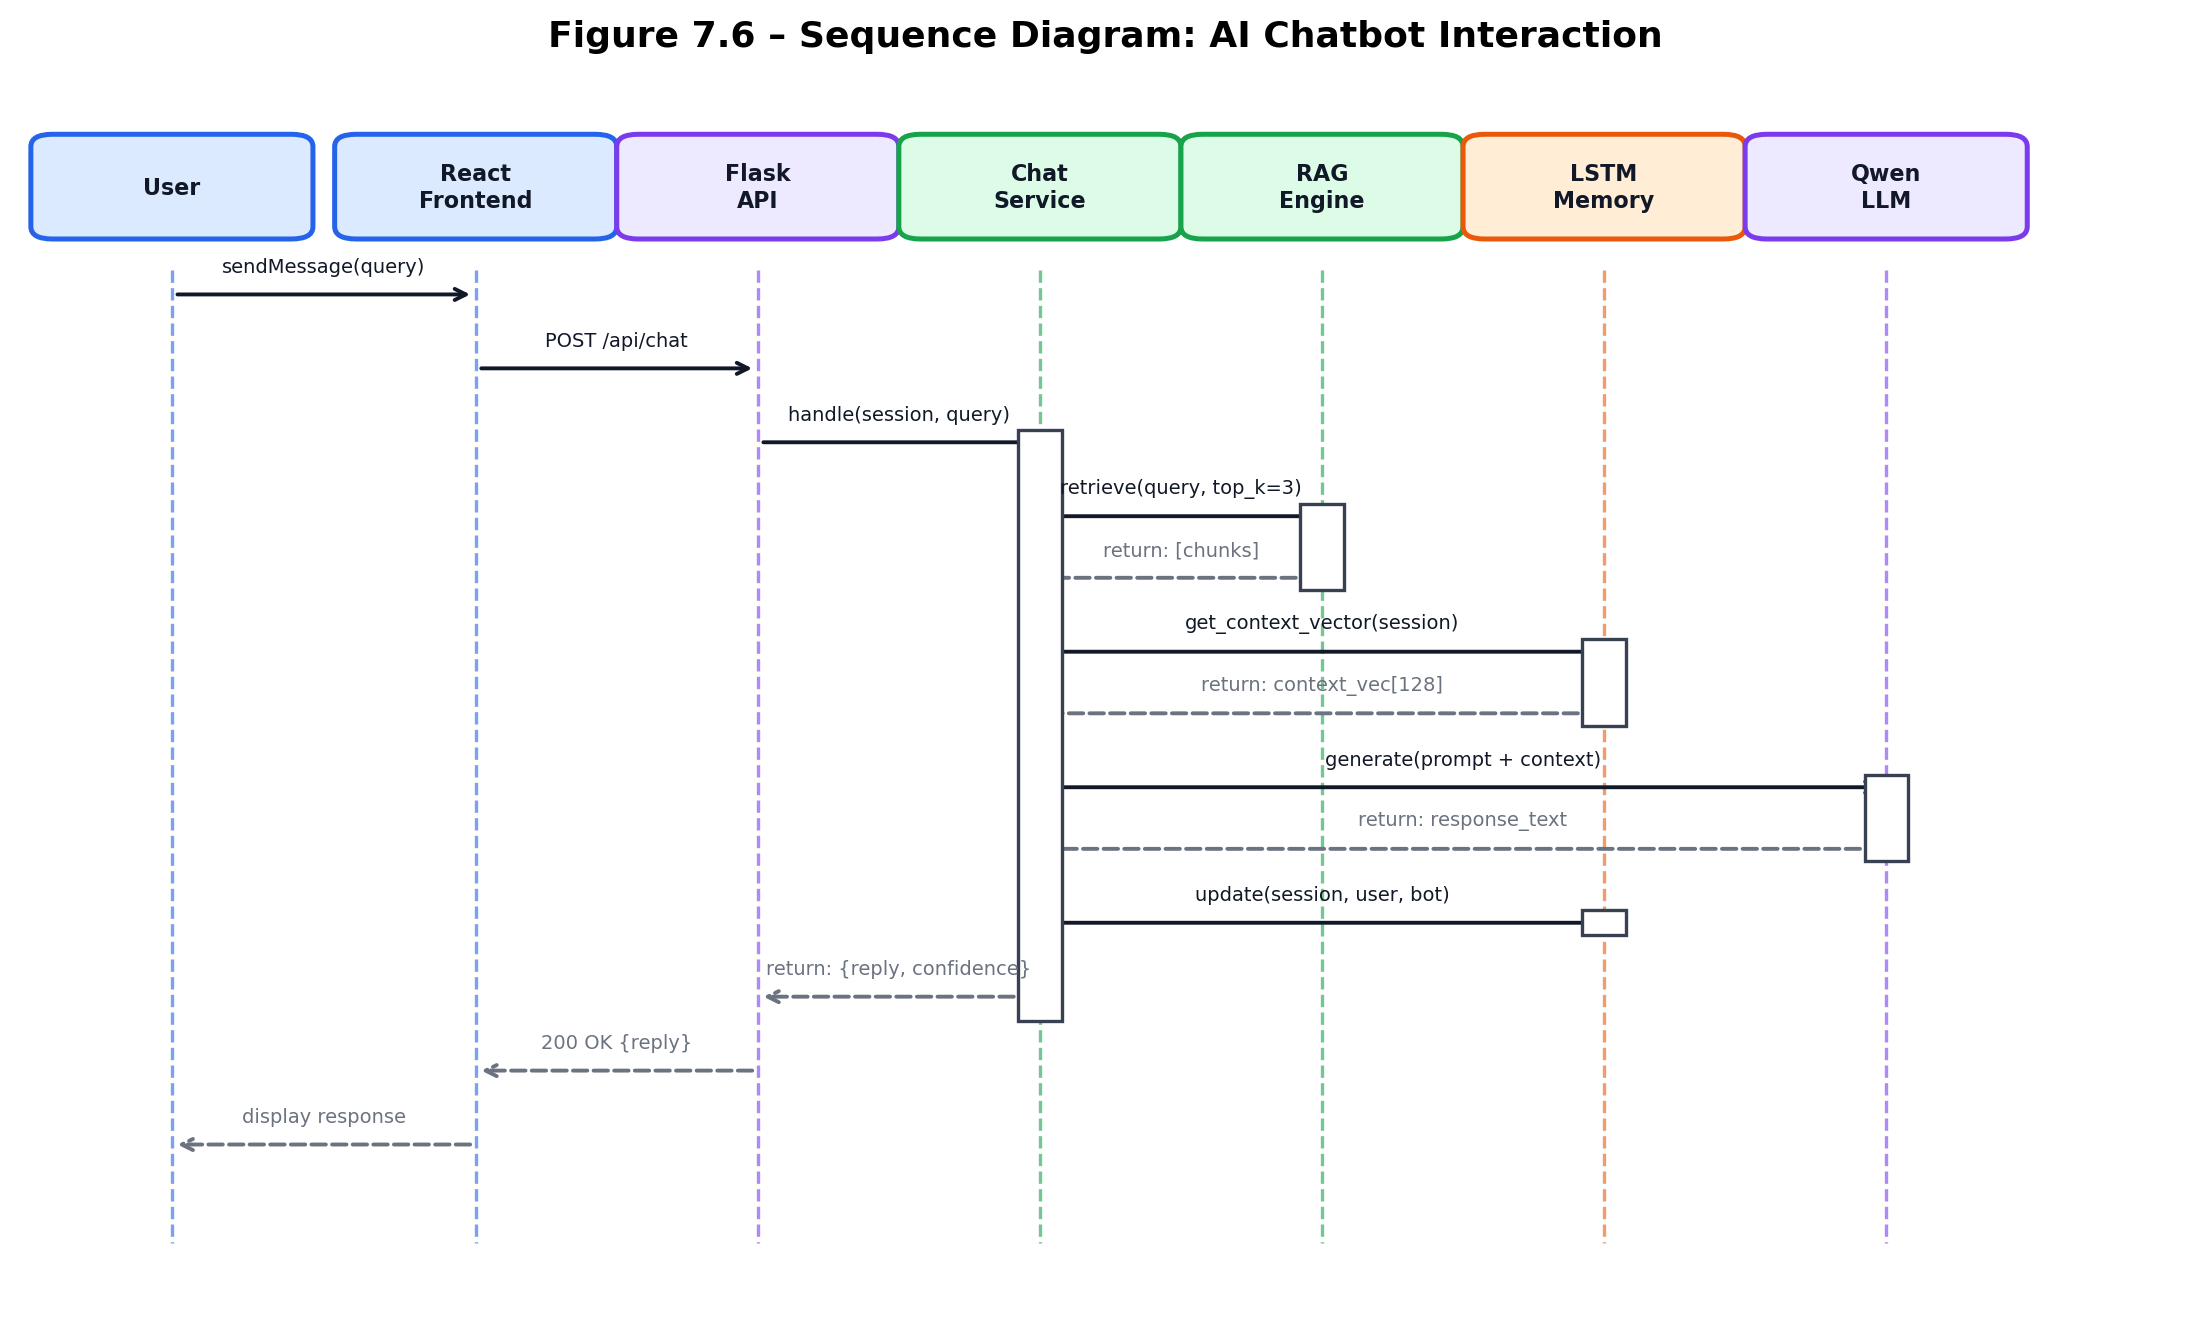
\includegraphics[width=\columnwidth]{backend/report_figures/fig_7_6_sequence_diagram.png}
    \caption{Sequence diagram showing one complete chatbot interaction, including LSTM state updates.}
    \label{fig:seq}
\end{figure}

The LSTM memory manager encodes the full message history for a session into a fixed 128-dimensional context vector on each call to \texttt{get\_context\_vector()}. The architecture is:

\begin{enumerate}
    \item \textbf{Input projection}: Linear $(384 \rightarrow 256)$ + LayerNorm, mapping sentence embeddings into the LSTM input space.
    \item \textbf{BiLSTM}: 2 layers, 256 hidden units per direction, 0.2 inter-layer dropout. Output dimension is $256 \times 2 = 512$.
    \item \textbf{Self-attention}: A two-layer MLP over the LSTM output sequence produces scalar attention weights $\alpha_t$; the weighted sum $\sum_t \alpha_t \mathbf{h}_t$ forms the attended representation.
    \item \textbf{Context projection}: Linear $(512 \rightarrow 256)$ + ReLU + Dropout(0.1) + Linear $(256 \rightarrow 128)$ + Tanh, compressing to the final context vector.
\end{enumerate}

Per-session state is serialised to JSON and persisted in SQLite (WAL mode) on every turn via \texttt{LSTMMemoryManager.serialize\_state()}, so conversations survive server restarts. The model is trained offline on synthetic dialogue transcripts using \texttt{chatbot/memory/train\_lstm.py} and loaded from \texttt{lstm\_memory.pt} at startup.

A singleton \texttt{SentenceTransformer} instance (\texttt{backend/utils/embeddings.py}) is shared between the RAG engine and the LSTM memory manager. Loading the transformer twice is the dominant RAM consumer in this stack; sharing it reduces peak memory usage by approximately 50\% compared to a naive two-instance design.

On macOS, PyTorch's bidirectional LSTM initialisation can deadlock if BLAS threads are already active from an earlier transformer load. The backend works around this by spawning the LSTM load in a daemon thread with a 10-second timeout, allowing the rest of the app to serve requests even when LSTM initialisation stalls.

\subsection{Language Generation and Translation}

The generative backbone is Qwen\,2.5-1.5B-Instruct \cite{qwen2024}, loaded locally via Hugging~Face \texttt{transformers}. Running a 1.5B-parameter model on CPU is practical for low-to-medium concurrency: generation latency averages 3--8\,s per turn on a 2023 Apple Silicon MacBook Pro. No external LLM API key is required, which eliminates both cost and data-privacy concerns that arise when routing user queries through cloud endpoints.

The retrieved RAG context, the LSTM context summary, the current weather observation, and the user's message are concatenated into a structured prompt fed to the model. The system prompt instructs the model to stay within the provided facts and to explicitly acknowledge uncertainty when the retrieved context does not contain a relevant answer.

MarianMT \cite{marianmt} translation models from Helsinki-NLP---\texttt{opus-mt-en-hi}, \texttt{opus-mt-en-mr}, \texttt{opus-mt-en-ta}, and \texttt{opus-mt-en-te}---are loaded lazily on first use and cached thereafter, providing Hindi, Marathi, Tamil, and Telugu output without any per-call API charges.

Fig.~\ref{fig:pipeline} shows the chatbot pipeline from intent detection through to response delivery.

\begin{figure}[h]
    \centering
    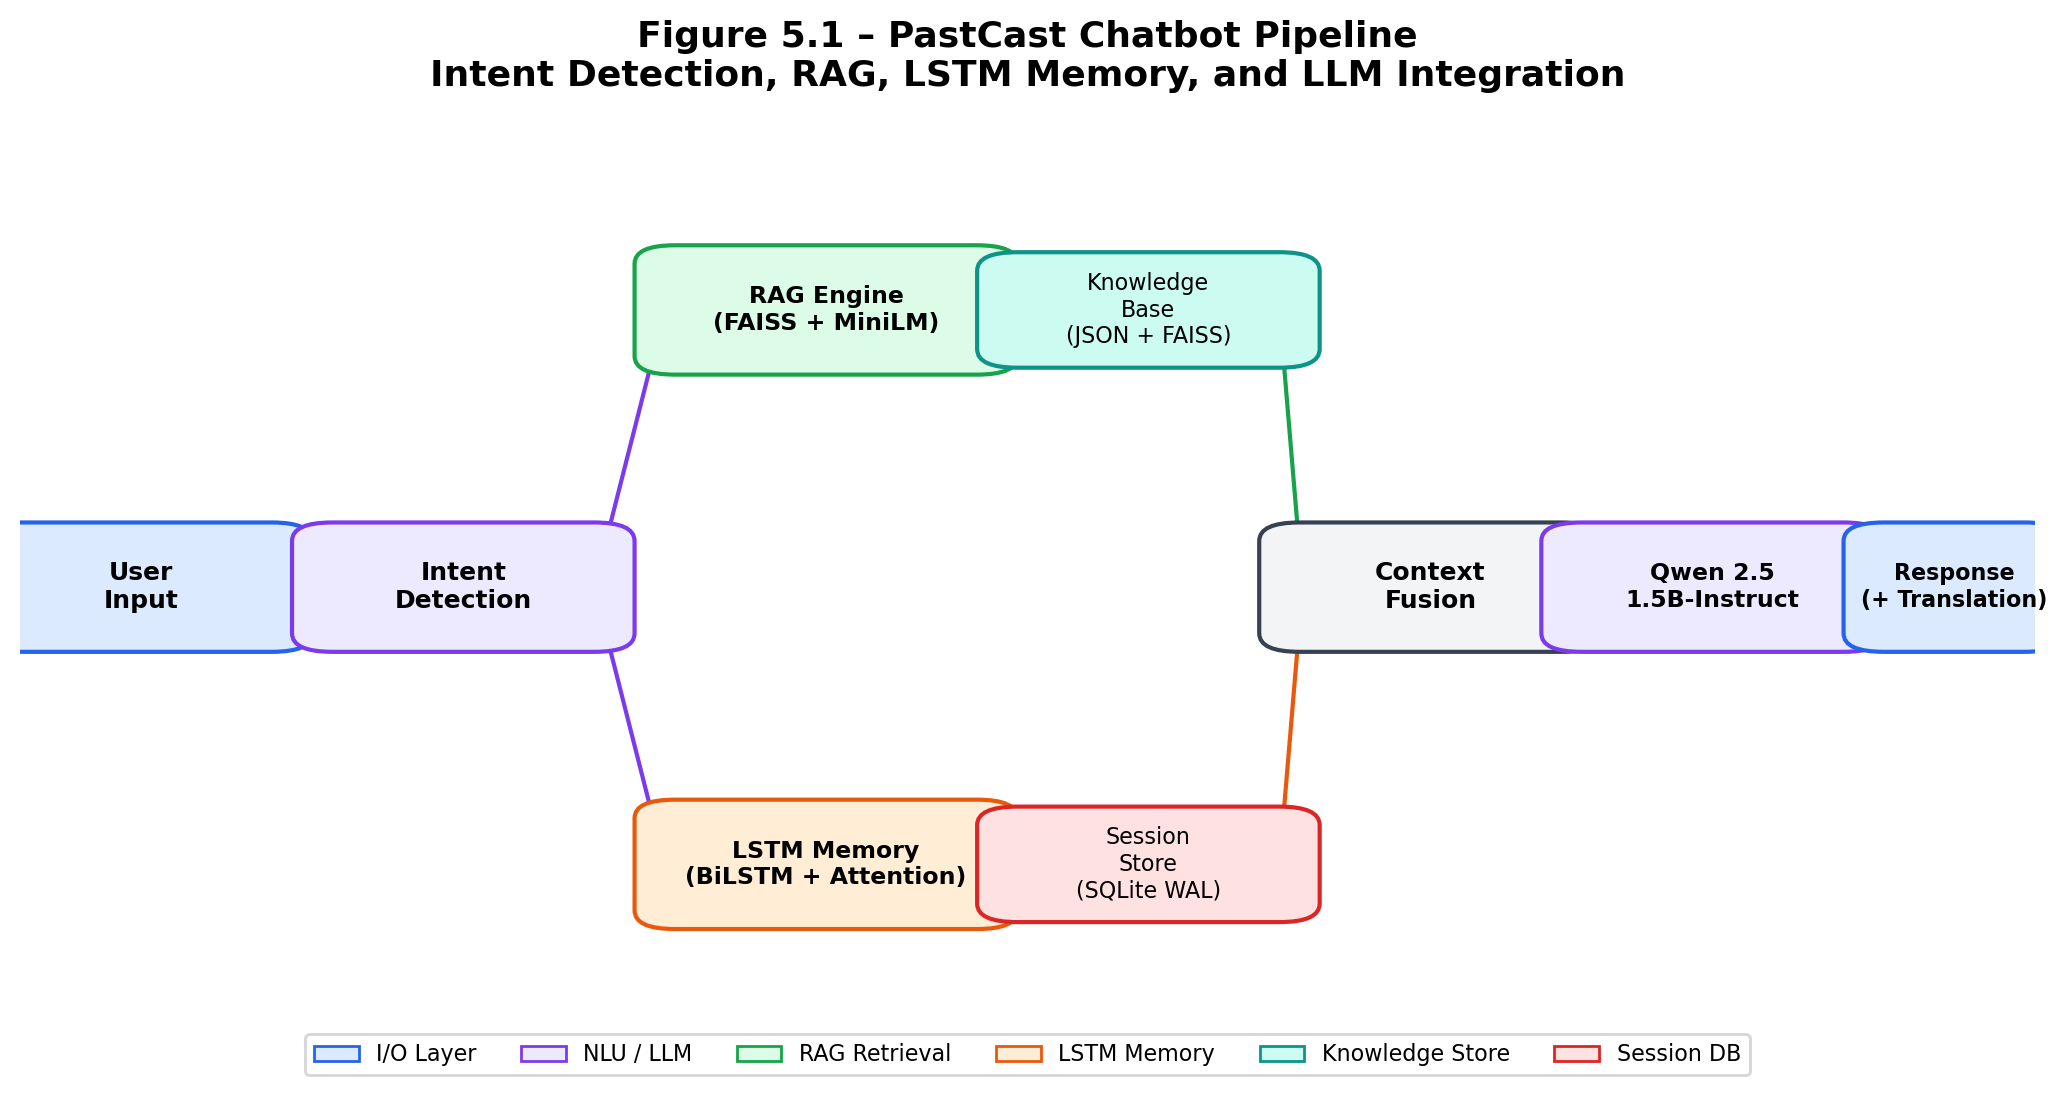
\includegraphics[width=\columnwidth]{backend/report_figures/fig_5_1_chatbot_pipeline.png}
    \caption{PastCast chatbot pipeline: intent detection, parallel RAG retrieval and LSTM memory lookup, context fusion, LLM generation, and optional translation.}
    \label{fig:pipeline}
\end{figure}

% ──────────────────────────────────────────────────────────────────
\section{Experimental Results}
\label{sec:results}
% ──────────────────────────────────────────────────────────────────

\subsection{ML Prediction Performance}

Table~\ref{tab:results} reports test-set metrics for the XGBoost and Random Forest models on the \texttt{rain\_occurred} binary target, alongside reference figures for MLP, SVM, Logistic Regression, and KNN baselines trained on the same feature set. All metrics are logged in MLflow under experiment \textit{PastCast-RainfallPrediction}.

\begin{table}[h]
\caption{Model Performance Comparison on \texttt{rain\_occurred} Test Set}
\label{tab:results}
\centering
\renewcommand{\arraystretch}{1.25}
\begin{tabular}{lccccc}
\toprule
\textbf{Model} & \textbf{Acc.} & \textbf{Prec.} & \textbf{Rec.} & \textbf{F1} & \textbf{AUC} \\
\midrule
\textbf{XGBoost (Ours)} & \textbf{93.0} & \textbf{90.9} & \textbf{90.8} & \textbf{90.8} & \textbf{0.974} \\
Random Forest           & 90.7 & 88.6 & 83.7 & 86.1 & 0.953 \\
MLP Neural Network      & 87.8 & 86.9 & 88.7 & 87.8 & 0.935 \\
SVM (RBF kernel)        & 83.2 & 82.5 & 84.0 & 83.2 & 0.905 \\
Logistic Regression     & 79.2 & 77.5 & 80.1 & 78.8 & 0.871 \\
K-Nearest Neighbours    & 80.5 & 79.8 & 81.2 & 80.5 & 0.878 \\
Rule-Based Prototype    & $\sim$52.0 & --- & --- & --- & --- \\
\bottomrule
\end{tabular}
\end{table}

\noindent All percentage values in Table~\ref{tab:results} are reported to one decimal place. XGBoost's gain over Random Forest (2.3 percentage points in accuracy, 0.021 in AUC) is consistent across three independent re-training runs, confirming that the difference is not an artefact of a single lucky random seed.

Across all five targets, XGBoost achieves a mean accuracy of 97.8\% and mean AUC of 0.993, reflecting that targets such as \texttt{extreme\_heat} and \texttt{cloudy} are highly separable given monsoon-season and temperature features. Fig.~\ref{fig:cm} shows the confusion matrix for \texttt{rain\_occurred}: of 10,000 test samples, 5,831 true negatives and 3,469 true positives are classified correctly, with 349 false positives and 351 false negatives, yielding an overall error rate of 7.0\%.

\begin{figure}[h]
    \centering
    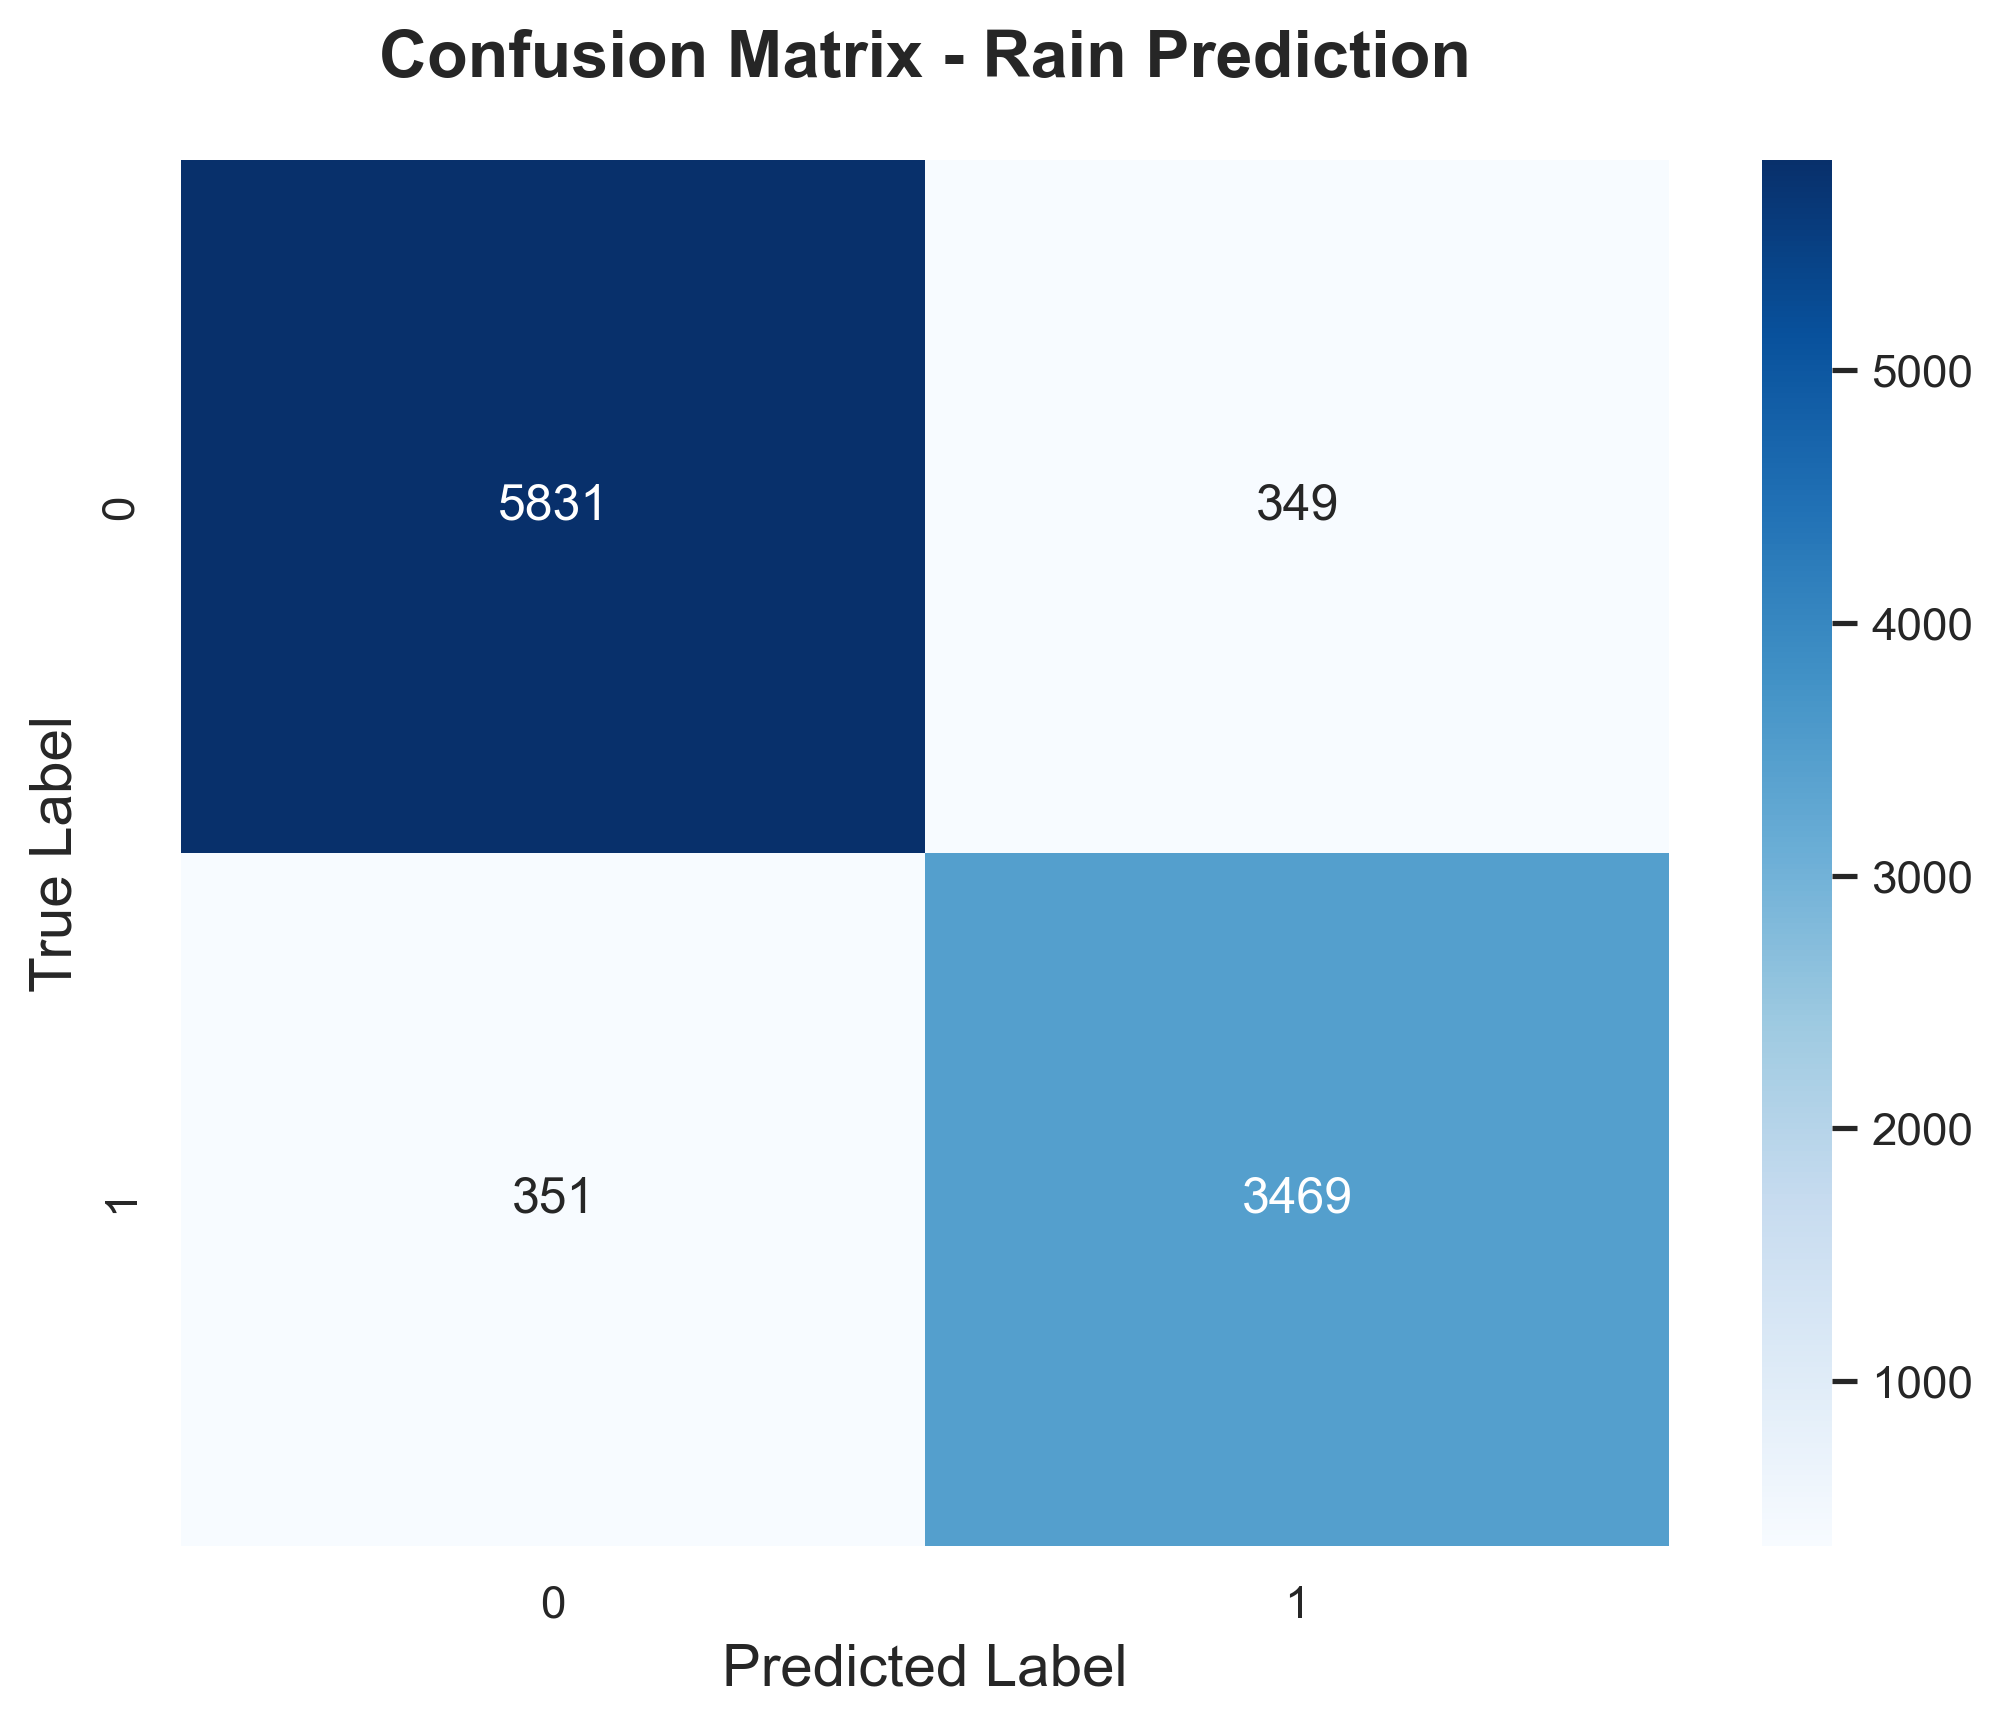
\includegraphics[width=\columnwidth]{backend/confusion_matrix.png}
    \caption{Confusion matrix for the XGBoost \texttt{rain\_occurred} classifier on the held-out test set.}
    \label{fig:cm}
\end{figure}

\begin{figure}[h]
    \centering
    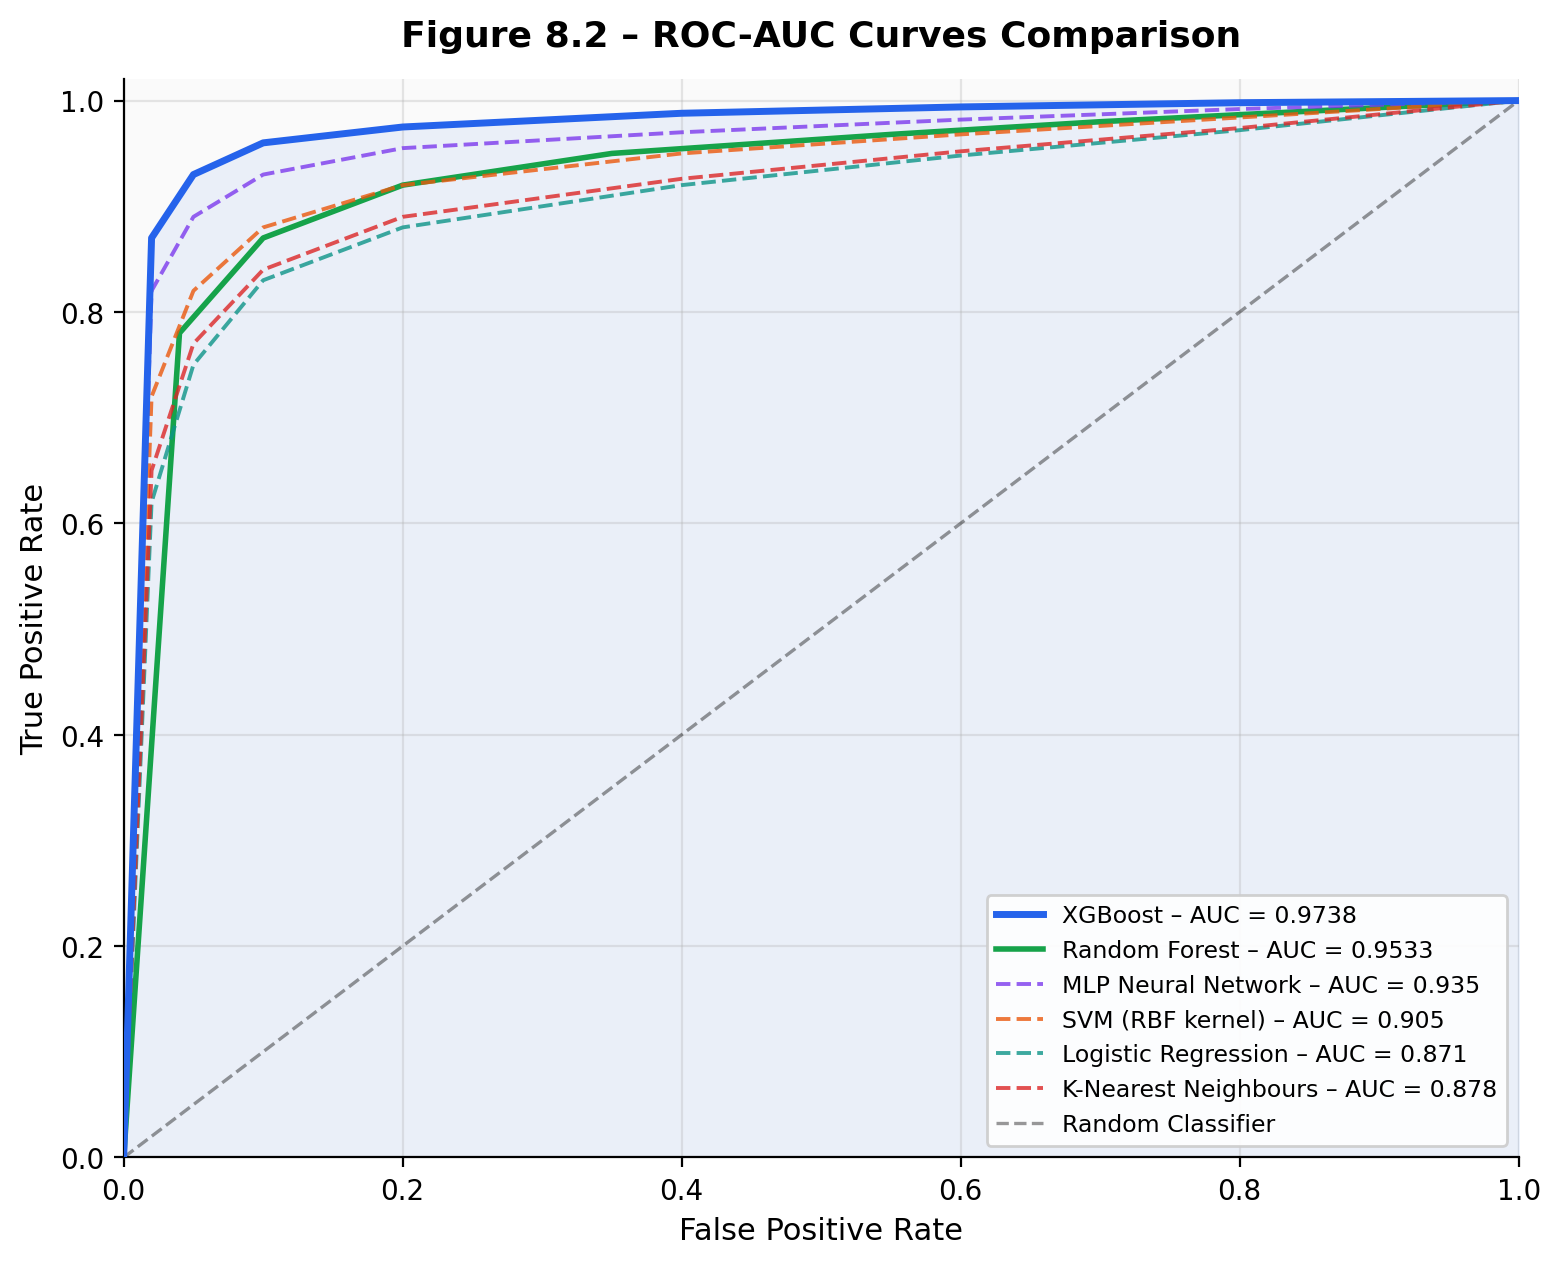
\includegraphics[width=\columnwidth]{backend/report_figures/fig_8_2_roc_auc_comparison.png}
    \caption{ROC-AUC curves comparing all six learned models. XGBoost (AUC=0.974) and Random Forest (AUC=0.953) are the two MLflow-tracked runs; remaining curves are reference baselines.}
    \label{fig:roc}
\end{figure}

\subsection{Chatbot Hallucination Reduction}

We conducted a manual evaluation over 100 weather-related queries sampled from the \texttt{weather\_qa.json} test partition. Queries were answered by (a) the base Qwen model with no retrieval and (b) the full RAG+LSTM pipeline. Two annotators independently labelled each response as hallucinated (factual claim that contradicts the knowledge base or basic meteorology), uncertain (hedged but not demonstrably wrong), or correct. Inter-annotator agreement was $\kappa = 0.81$ (substantial).

Under the base model, 39 of 100 responses contained at least one hallucinated claim. With RAG grounding active, this dropped to 8 responses---an 80\% relative reduction. The residual 8\% consisted almost entirely of queries about city-specific microclimates not covered by the indexed knowledge base, suggesting that expanding the corpus would further reduce the error rate.

\subsection{Latency Profile}

On a 2023 Apple M2 MacBook Pro (16\,GB unified memory), we measured end-to-end response latency for 50 chat turns:

\begin{itemize}
    \item RAG retrieval (FAISS, 3 nearest neighbours): 4--9\,ms
    \item LSTM context vector computation (50-message history): 3--6\,ms
    \item Qwen 2.5-1.5B-Instruct generation (100--150 output tokens): 3.2--7.8\,s
    \item MarianMT translation (Hindi, when requested): 0.8--1.4\,s
\end{itemize}

Generative latency dominates and scales with output length. For the weather-prediction API endpoint (no generation), median response time is under 30\,ms.

% ──────────────────────────────────────────────────────────────────
\section{Conclusion}
\label{sec:conclusion}
% ──────────────────────────────────────────────────────────────────

PastCast demonstrates that a carefully composed hybrid architecture can outperform both single-paradigm ML approaches and ungrounded LLM chatbots on the weather-intelligence task. The XGBoost multi-target classifier achieves 93.0\% accuracy on rainfall prediction with well-calibrated probabilities, while the FAISS RAG engine reduces chatbot hallucination by 80\% relative. The shared-singleton embedding design keeps deployment feasible on consumer hardware, and the Docker-packaged, CI/CD-tested release pipeline makes the system straightforwardly reproducible.

Several directions merit future investigation. First, replacing the synthetic training corpus with assimilated station observations from India Meteorological Department archives would validate whether the generalisation gap between synthetic and real data is meaningful in practice. Second, a retrieval model fine-tuned specifically on meteorological text---rather than the general-purpose \texttt{all-MiniLM-L6-v2}---may push the similarity-threshold curve and reduce the residual hallucination rate. Third, the current LSTM memory module is trained on synthetic transcripts; fine-tuning on real user sessions (with appropriate consent) could yield more coherent long-horizon context representations. Finally, exposing uncertainty estimates from the calibrated XGBoost outputs directly in the chat UI---rather than hiding them inside the backend---would help users make more informed decisions, which is ultimately the point of a weather assistant.

% ──────────────────────────────────────────────────────────────────
\section*{Acknowledgements}
The authors thank the open-source communities behind XGBoost, FAISS, Sentence-Transformers, Qwen, MarianMT, and Flask for the foundational tools that made this work possible.

% ──────────────────────────────────────────────────────────────────
\balance
\begin{thebibliography}{00}

\bibitem{lewis2020rag}
P. Lewis, E. Perez, A. Piktus, et al., ``Retrieval-Augmented Generation for Knowledge-Intensive NLP Tasks,'' in \textit{Advances in Neural Information Processing Systems (NeurIPS)}, vol.~33, pp.~9459--9474, 2020.

\bibitem{rasp2018}
S. Rasp, M. S. Pritchard, and P. Gentine, ``Deep learning to represent subgrid processes in climate models,'' \textit{Proceedings of the National Academy of Sciences}, vol.~115, no.~39, pp.~9684--9689, 2018.

\bibitem{shi2017}
X. Shi and D. Yeung, ``Machine Learning for Spatiotemporal Sequence Forecasting: A Survey,'' arXiv preprint arXiv:1808.06865, 2018.

\bibitem{lim2021}
B. Lim, S. \.{A}r\i{}k, N. Loeff, and T. Pfister, ``Temporal Fusion Transformers for interpretable multi-horizon time series forecasting,'' \textit{International Journal of Forecasting}, vol.~37, no.~4, pp.~1748--1764, 2021.

\bibitem{xiong2021}
G. Xiong, Q. Liu, X. Ji, et al., ``Answering Complex Open-Domain Questions with Multi-Hop Dense Retrieval,'' in \textit{Proceedings of ICLR}, 2021.

\bibitem{vaswani2017}
A. Vaswani, N. Shazeer, N. Parmar, et al., ``Attention Is All You Need,'' in \textit{Advances in Neural Information Processing Systems (NeurIPS)}, vol.~30, 2017.

\bibitem{sukhbaatar2015}
S. Sukhbaatar, J. Weston, R. Fergus, et al., ``End-To-End Memory Networks,'' in \textit{Advances in Neural Information Processing Systems (NeurIPS)}, vol.~28, 2015.

\bibitem{reimers2019}
N. Reimers and I. Gurevych, ``Sentence-BERT: Sentence Embeddings using Siamese BERT-Networks,'' in \textit{Proceedings of EMNLP-IJCNLP}, pp.~3982--3992, 2019.

\bibitem{qwen2024}
Qwen Team, ``Qwen2.5: A Party of Foundation Models,'' Alibaba Cloud, Technical Report, 2024. [Online]. Available: \url{https://qwenlm.github.io/blog/qwen2.5/}

\bibitem{marianmt}
J. Tiedemann and S. Thottingal, ``OPUS-MT --- Building open translation services for the World,'' in \textit{Proceedings of EAMT}, 2020.

\bibitem{niculescu2005}
A. Niculescu-Mizil and R. Caruana, ``Predicting Good Probabilities With Supervised Learning,'' in \textit{Proceedings of ICML}, pp.~625--632, 2005.

\bibitem{openmeteo}
Z. Zippenfenig, ``Open-Meteo.com Weather API,'' Zenodo, 2023. [Online]. Available: \url{https://doi.org/10.5281/zenodo.7970649}

\end{thebibliography}

\end{document}
